\section{Introducci'on}

La metamorfosis de im'agenes (en ingl'es, \textit{image morphing}) es una t'ecnica para transformar una imagen (la \textit{imagen origen}) en otra (la \textit{imagen destino}). Esta t'ecnica ha sido ampliamente utilizada en el 'ambito de la industria cinematogr'afica. Un ejemplo can'onico de su aplicaci'on puede verse en el video de la canci'on \textit{Black or White} de Michael Jackson, en el cual hay una secuencia de transformaciones entre las caras de personas de muy distintas caracter'isticas.

Diversos algoritmos para realizar esta metamorfosis han sido desarrollados, siendo el m'as b'asico aquel conocido como \textit{cross-dissolving}, que consiste en hacer desaparecer la imagen origen a medida que se hace aparecer la imagen destino, de forma gradual, creando un efecto de disoluci'on de ambas im'agenes. Concretamente, esta t'ecnica consiste en interpolar de a pares los colores de los p'ixeles de la imagen origen con los de la imagen destino, para luego variar el valor de la interpolaci'on a lo largo del tiempo.

\begin{figure}[H]
	\begin{center}
		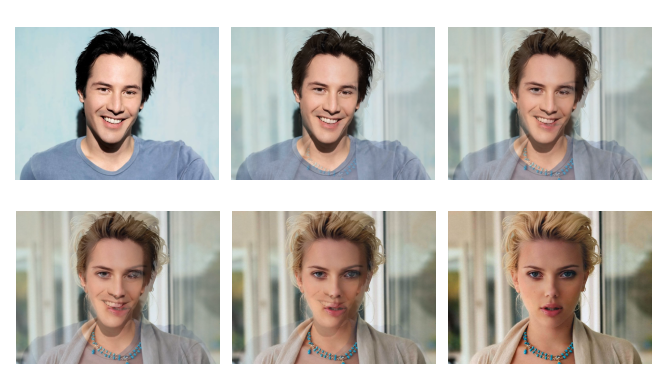
\includegraphics[scale=0.65]{imagenes/dissolving.png}
	\end{center}		
	\caption{Cross-dissolving}
	\label{fig1}
\end{figure}

Esta t'ecnica no resulta satisfactoria, puesto que la transformaci'on no es natural, en el sentido de que no sugiere que lo que ocurre es una metamorfosis. Esto se debe a que las caracter'isticas de la imagen origen no se transforman naturalmente en ciertas otras caracter'isticas de la imagen destino. Por esta raz'on, las t'ecnicas m'as elaboradas de image morphing emplean la deformaci'on de im'agenes (en ingl'es, \textit{image warping}) acompa\~{n}ado de un cross-dissolving, para obtener esa naturalidad buscada en la transformaci'on. La principal diferencia entre los distintos m'etodos de morphing est'a en la forma en que se mapean las caracter'isticas de la imagen origen en las de la imagen destino.

En este trabajo nos concentramos en la t'ecnica desarrollada por Beier y Neely, presentada en \cite{1}, que realiza el mapeo de caracter'isticas a trav'es de segmentos dirigidos (l'ineas rectas con principio, fin y sentido) en la imagen origen asociados a segmentos dirigidos en la imagen destino. Esto no s'olo determina c'omo deben ser transformados los puntos sobre esos segmentos, sino que tambi'en dan informaci'on sobre la transformaci'on de los puntos que los rodean. Implementamos una versi'on de este m'etodo basada en instrucciones SIMD, y la comparamos contra una versi'on tradicional, que realiza el procesamiento en serie, ganando, la primera, en t'erminos de tiempo de ejecuci'on, por un amplio margen. No tenemos registro de ninguna publicaci'on sobre una implementaci'on de este tipo, ni siquiera de los resultados de la vectorizaci'on de otros algoritmos de metamorfosis de im'agenes, con lo cual nuestro aporte es, en peque\~{n}a dosis, novedoso.

\begin{figure}[H]
	\begin{center}
		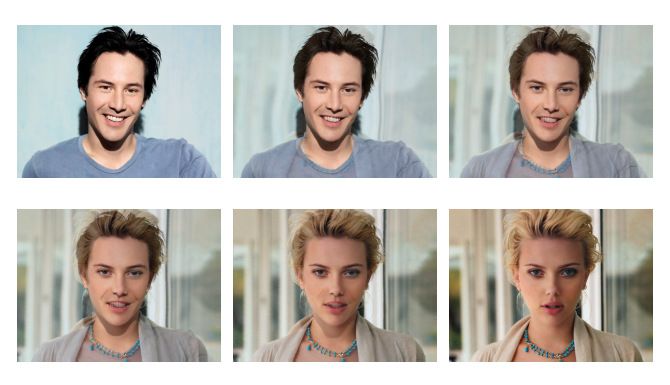
\includegraphics[scale=0.65]{imagenes/warping.png}
	\end{center}		
	\caption{Cross-dissolving con warping}
	\label{fig2}
\end{figure}

Organizamos esta exposici'on en cuatro partes. En primer lugar, proveemos un sencillo marco te'orico para comprender la matem'atica atr'as de esta t'ecnica. En segundo lugar, explicamos el algoritmo de Beier y Neely, con el m'aximo grado de detalle posible. En tercer lugar, desarrollaremos la vectorizaci'on realizada, contrastando esta implementaci'on contra la tradicional. Finalmente, presentamos los experimentos y, en base a ello, concluimos sobre la efectividad de la vectorizaci'on realizada.